\ifdefined\namedversion
\documentclass[manuscript,screen]{acmart}
\else
\documentclass[manuscript,screen,review,anonymous]{acmart}
\fi
\usepackage{amsmath,amssymb,booktabs,graphicx}
\setcopyright{none}
\settopmatter{printacmref=false}
\renewcommand\footnotetextcopyrightpermission[1]{}
\acmConference[FAccT 2027 submission]{Submitted for consideration at the ACM Conference on Fairness, Accountability, and Transparency}{2027}{Porto, Portugal}
\acmYear{2027}
\copyrightyear{2027}
\acmDOI{}
\acmISBN{}
\newtheorem{proposition}{Proposition}
\newtheorem{definition}{Definition}
\newcommand{\ind}{\mathbf{1}}
\title{Equal Quotas, Unequal Access: A Two-Ledger Audit of Multilingual Token Reservations}
\author{Shivam Gupta}
\affiliation{\institution{Independent Researcher}\city{Delhi}\country{India}}
\email{shivam1720406@gmail.com}
\begin{abstract}
Token quotas distribute access to language-model infrastructure, but the quantity reserved before admission can differ from the tokens charged after execution. We study how this accounting boundary changes multilingual access measurement. A pinned open-source gateway estimates input tokens as character count divided by four. Using 2,009 aligned FLORES-200 sentences in twelve languages and three tokenizers, we jointly measure admission, committed token usage, and quota feasibility. In a controlled burst experiment, this estimator admits 49.48\% of requests with cl100k\_base while committing 3.37 times the aggregate quota; one language-specific key commits 7.81 times its quota. Replacing the estimate with exact counts restores feasibility but yields a 45.80 percentage-point admission gap under equal token entitlements. Separate-data calibration of unequal token entitlements reduces that gap to 0.56 points at the same aggregate budget, while reducing total admitted requests by 40.4\%. We derive reservation-error bounds, an admission-ranking inversion witness, and exact finite-workload parity benchmarks that expose content-selection tradeoffs. Across 34,974,720 simulated admission decisions, 291,456 decisions also match executions of unchanged upstream Lua in Redis. The contribution is a reproducible audit of quota-mediated access and its accounting assumptions, rather than a new tokenizer or a measurement of deployed user harm. Capacity accounting, entitlement policy, and linguistic accessibility require separate evidence.
\end{abstract}
\begin{CCSXML}
<ccs2012><concept><concept_id>10002978.10003022.10003023</concept_id><concept_desc>Security and privacy~Access control</concept_desc><concept_significance>300</concept_significance></concept><concept><concept_id>10003120.10003121.10003126</concept_id><concept_desc>Human-centered computing~HCI theory, concepts and models</concept_desc><concept_significance>300</concept_significance></concept></ccs2012>
\end{CCSXML}
\ccsdesc[300]{Security and privacy~Access control}
\ccsdesc[300]{Human-centered computing~HCI theory, concepts and models}
\keywords{linguistic equity, algorithmic auditing, token quotas, admission control, multilingual access, AI gateways}
\begin{document}
\maketitle

\section{Introduction}
A multilingual service can advertise the same token quota to every customer and still give customers very different opportunities to complete comparable tasks. Tokenization disparities are an established reason: translations of the same content can require different numbers of model tokens~\cite{petrov2023,ahia-etal-2023-languages}. A second decision occurs outside the model. A gateway must decide whether to admit a request before execution provides final usage. That decision can depend on a reservation estimate rather than the tokenizer whose units define the quota. An audit that observes admissions without inspecting this accounting boundary can confuse additional access with additional unreserved consumption.

Consider two customers submitting translations of the same documents for semantic indexing. Their plans provide equal token quotas. The gateway estimates demand from text length, admits requests, and reconciles the estimate after completion. If the estimator undercounts one script, that customer can appear to receive more access while the service commits more tokens than the plan permits. Reconciliation corrects the ledger after the commitment; it cannot retroactively prevent the admission. Conversely, correcting the estimator can reduce measured access for that customer without changing the model, documents, nominal quota, or output quality. A comparative fairness claim therefore needs a common capacity constraint as well as a common task denominator.

This is a sociotechnical allocation question. The provider chooses the tokenizer, the reservation rule, the quota unit, and whether multilingual customers must bear the resulting differences. Equal payment or equal advertised entitlements need not amount to equal practical access. A resource accounting rule is necessary for operational protection, but it does not determine which entitlement policy is justified. Following critiques of abstraction in fair computing~\cite{selbst2019} and of underspecified language-technology harms~\cite{blodgett-etal-2020-language}, we explicitly separate three objects: the quantity a limiter reserves, the tokens the admitted workload requires, and the comparable tasks that customers can submit successfully.

We investigate this separation through an executable audit of one pinned LiteLLM limiter component~\cite{litellm}. The component provides a useful, inspectable case because it combines pre-call reservations, a character-based input estimate, atomic quota checks, and post-call reconciliation. Our controlled workloads contain aligned, published translations rather than generated approximations. We use input-only requests to isolate the input estimator from generation length. Three tokenizers expose how the same reservation rule behaves under different token units. We vary quota pressure, completion timing, task order, document length, and entitlement calibration. We also run the upstream admission and reconciliation Lua bodies in an isolated Redis instance.

The study addresses three questions. \textbf{RQ1:} How do reservation errors and settlement timing change multilingual admission and quota compliance? \textbf{RQ2:} What access differences remain after exact accounting restores compliance? \textbf{RQ3:} Can separately calibrated entitlements improve comparable access at a fixed aggregate budget, and what costs or assumptions does that improvement require?

Our contributions are: (1) a two-ledger audit specification linking translated task admission to reservation and true-token commitments; (2) sharp accounting bounds and finite-workload parity benchmarks, with proofs and exhaustive small-instance checks; (3) a versioned component study with real translations and tokenizers, including cross-runtime validation; and (4) a capacity-feasible entitlement calibration experiment that reports both access gains and request-throughput losses. The novelty sought is the joint measurement of linguistic access and reservation feasibility in an actual accounting path. We do not claim to discover tokenization inequity, invent fair scheduling, or establish that this effect occurs at any particular deployed customer service.

\begin{figure}[t]
\centering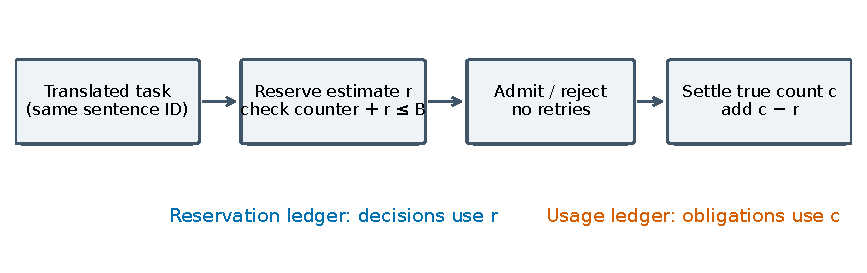
\includegraphics[width=.96\linewidth]{../figures/pipeline.pdf}
\caption{The audited boundary. Admission uses a reservation $r$, while the accepted request commits a true input cost $c$. Settlement adds $c-r$. The experiment controls when settlement occurs; it does not run model inference.}
\Description{A translated task is estimated, checked against a quota, admitted or rejected, and then reconciled using actual token count. Admission and usage use different ledgers.}
\label{fig:pipeline}
\end{figure}

\section{Related Work and Contribution Boundary}
\paragraph{Language representation and tokenization.}
Joshi et al.~\cite{joshi-etal-2020-state} document unequal language representation in NLP. Rust et al.~\cite{rust-etal-2021-good} investigate tokenizer quality in multilingual models. Petrov et al.~\cite{petrov2023} show that translated text has unequal token lengths and discuss resulting price, latency, and context inequalities. Ahia et al.~\cite{ahia-etal-2023-languages} examine language-dependent commercial tokenization costs. These studies establish why tokens are not a neutral unit of comparable linguistic service. We reuse that premise rather than present token-length ratios as a new discovery. Our outcome is the admission decision made by an estimator whose units can differ from those charged to the quota, including how settlement timing changes the comparison.

\paragraph{Fair LLM serving.}
Sheng et al.~\cite{sheng2024} define token-cost-based serving fairness and introduce the Virtual Token Counter scheduler. FairServe~\cite{khan2024} considers heterogeneous applications and interactions and develops application-aware throttling and weighted scheduling. These are important precedents for adapting service units to heterogeneous demand. They study allocation and scheduling among clients; they do not provide the translated-workload, character-estimator, reservation-versus-commitment audit performed here. Our calibrated quota allocation is a conventional proportional weighting baseline. It is not a replacement for VTC, and we do not compare its quality to a GPU scheduler on an input-only quota experiment.

\paragraph{Operational accounting.}
LiteLLM documentation describes reservation and reconciliation~\cite{litellmdocs}. Kong documentation distinguishes response-based counting from request-prompt counting~\cite{kong}, illustrating that admission boundaries vary across gateways. Those documents motivate checking the implementation rather than treating ``tokens per minute'' as a complete behavioral specification. Our runtime findings apply to the extracted LiteLLM components and tested configuration. We have not executed Kong or audited its estimator. The accounting inequalities below are elementary conservation results, not new general results in queueing theory.

\paragraph{Normative framing.}
Selbst et al.~\cite{selbst2019} explain why fairness interventions can fail when their abstraction boundary excludes institutions and social actors. Blodgett et al.~\cite{blodgett-etal-2020-language} call for specifying the social mechanisms and harms behind NLP bias claims. We operationalize these cautions: translated admission parity is a declared service objective, not a universal definition of fairness. We distinguish a language's script from an individual's identity, nominal quota from actual entitlement, and an executable failure mechanism from an estimate of its social prevalence. The contribution is an audit across these boundaries, with explicit costs and restricted claims.

\section{Setting, Estimands, and Accounting}
There are $L$ language-specific test keys and $n$ aligned tasks per key. Task $i$ has one published version in each language $\ell$. Let $c_{i\ell}>0$ be its exact input-token count under the tokenizer being evaluated, $r_{i\ell}>0$ its pre-call reservation, and $B_\ell$ its key's quota during one window. We impose no request-count or concurrency limit in the experiment. Requests rejected by this quota are not retried. There is no shared parent quota in the primary test; the aggregate budget $B_{\mathrm{tot}}=\sum_\ell B_\ell$ permits like-for-like comparison of entitlement policies.

At admission time, a key's counter contains settled true usage plus reservations for admitted requests that have not settled. A request is admitted when its counter plus $r_{i\ell}$ is at most $B_\ell$. An admission increases the counter by $r_{i\ell}$. Completion changes it by $c_{i\ell}-r_{i\ell}$. This matches the tested atomic check and guarded reconciliation logic, within one unexpired window. We call $\sum_{i\in A_\ell}r_{i\ell}$ the reservation sum of a selected batch and $U_\ell=\sum_{i\in A_\ell}c_{i\ell}$ its committed true-token demand. ``Committed'' is deliberate: counts are computed exactly, but no inference consumes the associated resources in this audit.

\begin{definition}[Audit outcomes]
For admitted set $A_\ell$, coverage is $a_\ell=|A_\ell|/n$. The access gap is $G=\max_\ell a_\ell-\min_\ell a_\ell$. Aggregate quota utilization is $V=\sum_\ell U_\ell/B_{\mathrm{tot}}$; a value above one is aggregate overcommitment. Per-key quota violation is captured by $V_{\max}=\max_\ell U_\ell/B_\ell$. Request throughput is $\sum_\ell |A_\ell|$, not tokens per second.
\end{definition}

A low gap can describe equally poor access. We therefore report minimum coverage, mean coverage, and the usage ratios alongside $G$. Likewise, $V\leq1$ does not imply every key respects its quota; $V_{\max}$ detects offsetting under- and overcommitment. Tokens are the contractual accounting unit in this experiment, not a direct measure of GPU time, monetary expense, energy, or welfare.

\subsection{Why Equal Tokens Is a Policy Choice}
The aligned task denominator asks a bounded question: how many versions of the same source tasks can a customer submit? It controls content more closely than comparing unrelated language corpora. It does not establish that all translations are equivalent in difficulty or downstream utility. FLORES-200 is a machine-translation evaluation corpus~\cite{flores,nllb2024}; its published text permits an input-accounting test, not a judgment about every language community's needs.

Equal token quotas can be justified when the product explicitly sells tokenizer units and customers understand the differences. Equal comparable-task access is another objective, relevant to a service promising multilingual document processing. Neither follows automatically from the other. Our calibration baseline chooses the latter objective while preserving the aggregate token budget. It transfers token entitlements toward languages whose observed translations require more tokens. The experiment makes that redistribution visible rather than describing a correction to token counting as a complete fairness remedy.

\section{Reservation Error and Feasible Parity}
\subsection{Accounting Bounds and an Inversion Witness}
Let $S\geq0$ be settled usage at the beginning of a batch, and let $A$ denote requests admitted before any request in that batch settles. Write $E_+(A)=\sum_{i\in A}(c_i-r_i)_+$, with $(x)_+=\max(x,0)$.

\begin{proposition}[Reservation-error certificate]\label{prop:error}
If the admission rule accepts only when the resulting reservation counter is at most $B$, then after settling a nonempty admitted batch,
\begin{equation}
S+\sum_{i\in A}c_i\;\leq\;B+E_+(A).\label{eq:error}
\end{equation}
The bound is attainable. If $r_i\geq c_i$ for every request, admitted true usage never exceeds $B$. Conversely, a guarantee of compliance for every nonnegative quota and workload requires $r_i\geq c_i$ for each admissible request.
\end{proposition}
\begin{proof}
At the final admission, $S+\sum_{i\in A}r_i\leq B$. Add $\sum_{i\in A}(c_i-r_i)$ and bound each term by its positive part. Equality is possible when reservations fill the budget and every error is nonnegative. Conservative reservations preserve the invariant ``settled true usage plus outstanding reservations is at most $B$'': admission checks it and settlement cannot increase it. For necessity, choose a request with $c_i>r_i$, an empty counter, and $B=r_i$. The request is admitted but its true demand exceeds $B$.
\end{proof}

This necessity is a uniform guarantee, not a statement that any underestimation must violate any particular quota. With serial settlement, a first crossing can exceed $B$ by at most the positive error of its final admitted request. No later request can be admitted once the settled counter is above $B$. With burst settlement, many errors accumulate before feedback becomes effective. The latency of accounting, even with atomic admission checks, is therefore a material audit parameter.

\begin{proposition}[Admission ranking can invert]\label{prop:invert}
For two keys, $N$ identical tasks per key, a common quota $B$, constant reservations $r_A,r_B$, and no settlement until all admissions finish, each admitted count is $\min(N,\lfloor B/r_\ell\rfloor)$ for key $\ell\in\{A,B\}$. Thus $r_B<r_A$ can make $B$'s observed admission larger even when $c_B>c_A$, reversing the ranking under exact counting.
\end{proposition}
\begin{proof}
The admission counter increases by the constant reservation for each accepted request. It permits exactly the stated number. With $N=10$, $B=16$, $(c_A,c_B)=(4,8)$ and $(r_A,r_B)=(4,2)$, estimated accounting admits $(4,8)$ requests and commits $(16,64)$ tokens. Exact accounting admits $(4,2)$ requests and commits $(16,16)$ tokens.
\end{proof}

The witness does not say token inequality is new. It shows why comparing access across accounting policies without checking capacity can reverse the interpretation. Our empirical analogue is a compact script whose character estimate is low while its exact token cost is relatively high.

\subsection{Two Exact Offline Benchmarks}
We use two finite-workload benchmarks to distinguish attainable access from content-selection artifacts. Pool the token budget across the $L$ keys, and fix a common task order $\pi$. Define
\begin{equation}
K_{\mathrm{prefix}}=\max\left\{k:\sum_{j=1}^k\sum_{\ell=1}^L c_{\pi(j),\ell}\leq B_{\mathrm{tot}}\right\}.\label{eq:prefix}
\end{equation}
This is the largest common prefix of identical task IDs that can be admitted in every language at the pooled budget. All costs are positive, so prefix sums are increasing and the optimum is exact. It is an offline common-progress benchmark, not a deployable mechanism for identifying translations in arbitrary customer traffic. Its per-key quotas can be set to the corresponding prefix costs, preserving the total resource constraint.

A less restrictive benchmark permits each language to choose different tasks. Let $c_{(j),\ell}$ be that language's $j$th smallest cost. Then
\begin{equation}
K_{\mathrm{count}}=\max\left\{k:\sum_{\ell=1}^L\sum_{j=1}^k c_{(j),\ell}\leq B_{\mathrm{tot}}\right\}.\label{eq:count}
\end{equation}
\begin{proposition}[Equal-count feasibility]\label{prop:frontier}
There exists a resource-feasible selection admitting at least $k$ tasks in each language if and only if the cost sum in Equation~\eqref{eq:count} is at most $B_{\mathrm{tot}}$. Consequently $K_{\mathrm{prefix}}\leq K_{\mathrm{count}}$.
\end{proposition}
\begin{proof}
Every selection containing at least $k$ items from a language costs at least the sum of its $k$ cheapest items. Summing proves necessity. Selecting those items in each language proves sufficiency. A feasible common prefix is a feasible equal-count selection, proving the final inequality.
\end{proof}

Sorting gives an $O(Ln\log n)$ certificate and a witness selection. The difference between these frontiers is substantively important: a quota allocator can report excellent count parity by disproportionately selecting short or inexpensive content. Such a policy need not preserve comparable task identity or meet the needs of customers with long documents. We report both frontiers and use neither as evidence of equitable service in deployment.

\subsection{A Separately Calibrated Entitlement Baseline}
Let $\widehat\mu_\ell$ be the mean true-token demand of language $\ell$ on the separate development split. Allocate
\begin{equation}
B_\ell\approx B_{\mathrm{tot}}\frac{\widehat\mu_\ell}{\sum_m\widehat\mu_m},\label{eq:cal}
\end{equation}
using largest-remainder integer apportionment so the quotas sum exactly to $B_{\mathrm{tot}}$. Admission then reserves exact input-token counts. If task costs were constant at their calibration means, all unsaturated keys would admit approximately the same number of tasks, with at most integer rounding effects. In heterogeneous held-out workloads, no exact parity guarantee follows. Sampling error, domain shift, and order effects must be measured.

This is a deliberately simple audit intervention. It uses established proportional weighting rather than a novel allocation algorithm. It tests whether the observed access difference is addressable by changing entitlements under a fixed aggregate budget, while keeping accounting safe. It also exposes the opportunity cost: moving quota away from cheaper languages can reduce the total number of accepted requests. Language labels are known experimental metadata; a deployment would need a justified, privacy-aware way to define and assign the relevant service class.

\section{Implementation and Experimental Protocol}
\subsection{Pinned Component and Execution Scope}
We freeze LiteLLM at commit \texttt{e0398455d09f} (full revision in the artifact). In \texttt{parallel\_request\_limiter\_v3.py}, the input estimator counts selected request characters and returns $\max(1,\lfloor\mathrm{characters}/4\rfloor)$ for nonempty text. Its embedding branch assigns zero output reservation. The Lua admission script checks proposed increments atomically across descriptors; the reconciliation script applies a signed delta only to the expected active window~\cite{litellm}. We extract these bodies from the vendored source without modifying their computation. An AST harness executes the relevant estimator methods on plain input strings and verifies their output against the formula used in the replay.

The harness does not instantiate the full HTTP proxy, provider adapter, database, router, or model. It omits chat message serialization, tools, multimodal input, cache discounts, streaming, and Google-native request translation. Source-defined behavior for those paths is not inferred from this experiment. We also do not assert that every LiteLLM configuration uses the tested path, or that the development-marked component has a particular deployment prevalence.

For conformance, an isolated Redis server executes the extracted admission and window-guarded settlement scripts on two full held-out task permutations for every tokenizer, exact versus character reservations, and serial versus full-burst settlement. The simulator's Boolean admission arrays and final true-usage counters must agree exactly. Redis test windows are configured to 3,600 seconds to avoid expiry during the test process; primary simulations represent a single window with no expiry. This changes the window parameter, not the Lua source. It tests accounting semantics within a window rather than time-to-reset or distributed expiry behavior.

\subsection{Data and Tokenizers}
The original FLORES-200 release contains aligned published translations and is distributed under CC BY-SA 4.0~\cite{flores}. We use all 997 development and 1,012 development-test sentences for each of twelve language-script codes: English, French, German, Spanish, Modern Standard Arabic, Hindi, Bengali, simplified Chinese, Japanese, Swahili, Telugu, and Burmese. These span different scripts and resource contexts; they are a purposive audit set rather than a sample weighted by world population or customer demand. Sentence identity is preserved across languages. No original text is republished in the code repository; the artifact provides retrieval instructions and hashes.

We count ordinary text with \texttt{cl100k\_base} and \texttt{o200k\_base} from tiktoken~\cite{tiktoken}, and the Qwen2.5 tokenizer at revision \texttt{060db6499f32} (full revision in the artifact)~\cite{qwen}. We disable special-token insertion. The audit therefore has 24,108 language-specific texts and 72,324 exact tokenizer evaluations. These are tokenizer evaluations, not 72,324 model queries. A secondary document-length check concatenates consecutive groups of four sentences with newlines: 249 calibration and 253 held-out documents per language, dropping one unmatched calibration remainder sentence. We record hashes, package versions, token counts, and the upstream source revision.

\subsection{Conditions and Baselines}
For each tokenizer, equal-key quota is $B=\lfloor f\sum_i c_{i,\mathrm{English}}\rfloor$, with $f\in\{0.25,0.5,0.75\}$. Each policy receives the same aggregate $12B$. English anchors the experimental load; it is not used to estimate the calibrated language weights or proposed as a normative reference population. The central condition is $f=0.5$. We compare four policies:
\begin{enumerate}
\item \textbf{Chars/4:} the pinned character estimator with equal per-key token quotas.
\item \textbf{Exact:} exact input counts with equal per-key quotas.
\item \textbf{Bytes:} UTF-8 byte length as a conservative reservation with equal quotas. For the tested byte-based tokenizers and ordinary strings, each token consumes at least one byte; empirically we verify $c\leq r$ for every text. This is not a guarantee for arbitrary tokenization or multimodal serialization.
\item \textbf{Calibrated:} exact counts and Equation~\eqref{eq:cal}, using only development-split means.
\end{enumerate}

All languages use the same sentence permutation for a given seed. We run seeds 100--129 without selecting favorable orders. In serial settlement, each admitted request settles before the next one is considered. In full-burst settlement, all requests are considered before any settlement; this is a concurrency stress case. At the central budget we also settle in blocks of eight and 64 requests. The primary matrix contains 2,880 complete replays and 34,974,720 individual admission decisions. These repeated decisions reuse the same corpus and are not independent observations of people or services.

A local prospective protocol was committed before counts and replay outcomes were generated. It was not publicly preregistered. The main matrix, language set, tokenizers, and seed range were fixed there. The intended 50\% English sensitivity was implemented as an entitlement-priority stress case with balanced demand: English receives half the aggregate quota, and the remaining quota is split among other languages by calibration cost. It is not a measured skewed-traffic experiment. We report this deviation rather than reinterpret it as an external-validity test.

\subsection{Uncertainty and Verification}
Order summaries average all thirty permutations. To assess sensitivity to corpus composition, we perform 1,000 paired sentence bootstrap replicates per tokenizer at the central burst condition, resampling aligned sentence IDs across all languages together. Calibration weights and quotas remain fixed, and the same resampled tasks and order are used for each compared policy. Percentile intervals use the 0.8333rd and 99.1667th percentiles: a Bonferroni adjustment across the three tokenizer-specific comparisons for each reported statistic. These are sensitivity intervals conditional on the benchmark's sampling interpretation, not population-level uncertainty about language communities. The interval family does not cover all descriptive endpoints simultaneously.

Eight test functions check the extracted estimator on varied scripts, 1,000 apportionments, conservative-reservation invariants, reservation-error bounds, the inversion witness, prefix feasibility, and exhaustive enumeration of equal-count selections in forty small instances. Complete Redis conformance is required separately. The code uses integer token ledgers; only apportionment weights and descriptive statistics use floating-point arithmetic.

\section{Results}
\subsection{RQ1: Admission Without Capacity Is a Misleading Comparison}
Table~\ref{tab:main} reports every tokenizer and policy in the central burst condition. The character estimator admits the most requests, but its committed usage exceeds the aggregate budget for all three tokenizers: $3.367\times$ for cl100k\_base, $1.517\times$ for o200k\_base, and $2.686\times$ for Qwen2.5. The maximum per-key ratio reaches $7.813\times$, $3.216\times$, and $6.103\times$, respectively. These comparisons cannot be interpreted as more efficient capacity-feasible admission.

\begin{table}[t]
\centering\small\begin{tabular}{llrrrr}\toprule
Tokenizer & Policy & Admitted (\%) & Gap (pp) & Usage / budget & Max. key ratio\\\midrule
cl100k\_base & Chars4 & 49.48 & 66.25 & 3.367 & 7.813\\
 & Exact & 22.19 & 45.80 & 0.999 & 1.000\\
 & Bytes & 7.20 & 8.28 & 0.393 & 0.676\\
 & Calibrated & 13.22 & 0.56 & 0.999 & 1.000\\
\midrule
o200k\_base & Chars4 & 49.02 & 66.62 & 1.517 & 3.216\\
 & Exact & 33.95 & 34.32 & 1.000 & 1.000\\
 & Bytes & 7.12 & 8.19 & 0.205 & 0.288\\
 & Calibrated & 31.45 & 1.03 & 1.000 & 1.000\\
\midrule
Qwen2.5 & Chars4 & 50.14 & 65.71 & 2.686 & 6.103\\
 & Exact & 26.97 & 44.59 & 0.999 & 1.000\\
 & Bytes & 7.31 & 8.45 & 0.325 & 0.544\\
 & Calibrated & 16.24 & 0.76 & 0.999 & 1.000\\
\bottomrule\end{tabular}

\caption{Central condition: equal translated demand, $f=0.5$, full burst, thirty task orders. ``Usage'' is exact committed input-token demand. Exact, Bytes, and Calibrated respect each key's quota; Chars/4 does not. Gap is maximum minus minimum language coverage in percentage points. Calibrated changes entitlements while preserving the total quota.}
\label{tab:main}
\end{table}

Figure~\ref{fig:admission} makes the language pattern visible. With cl100k\_base, Chars/4 admits all Chinese requests and 98.10\% of Japanese requests, compared with 41.86\% of English requests. Yet their exact committed-demand ratios are about 3.739, 4.445, and 0.834, respectively. Under exact reservations and the same per-key quotas, Chinese and Japanese coverage falls to 26.88\% and 22.13\%, while English coverage is 50.13\%. This is the empirical admission-ranking inversion in Proposition~\ref{prop:invert}. The estimate favors short character representations without guaranteeing small true-token demand.

Burmese illustrates a different aspect of the same accounting failure. Its character estimator admits 33.75\% of requests in the central cl100k\_base condition, but commits $7.813\times$ the key's quota. Exact counting admits 4.32\%. High overcommitment is therefore not synonymous with high absolute admission; both text length and tokenizer expansion matter. A single disparity number would obscure the mechanism.

\begin{figure}[t]
\centering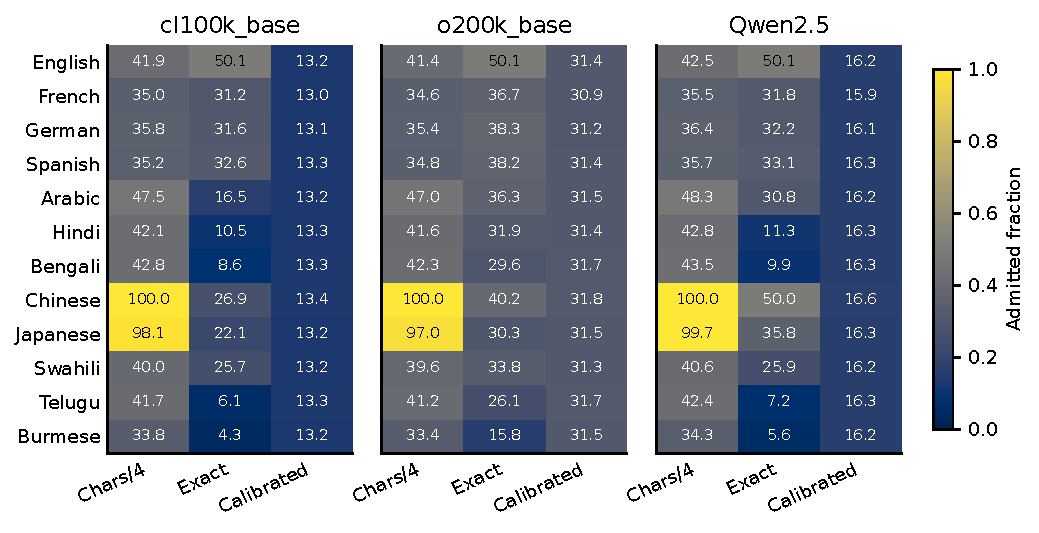
\includegraphics[width=.98\linewidth]{../figures/admission.pdf}
\caption{Mean language-specific admitted percentages in the central full-burst condition. The same tasks and quotas are used within each tokenizer. Chars/4 columns violate the capacity constraint; exact and calibrated columns respect it. Calibration reduces access gaps by reallocating token entitlements, not by improving the tokenizer.}
\Description{Three heatmaps show twelve languages under character estimates, exact reservations and calibrated quotas. Chinese and Japanese have high admissions under character estimates. Calibrated quotas bring coverage close together for each tokenizer.}
\label{fig:admission}
\end{figure}

Settlement substantially changes overcommitment (Figure~\ref{fig:error}). For cl100k\_base, aggregate usage ratios under Chars/4 are 1.003, 1.022, 1.142, and 3.367 for settlement blocks of one, eight, 64, and 1,012. Corresponding maximum key ratios are 1.013, 1.102, 1.497, and 7.813. Serial reconciliation limits accumulated reservation error; it does not make the estimate a valid worst-case reservation. The two newer tokenizer units have smaller or different errors, but retain the dependence on accounting delay.

\begin{figure}[t]
\centering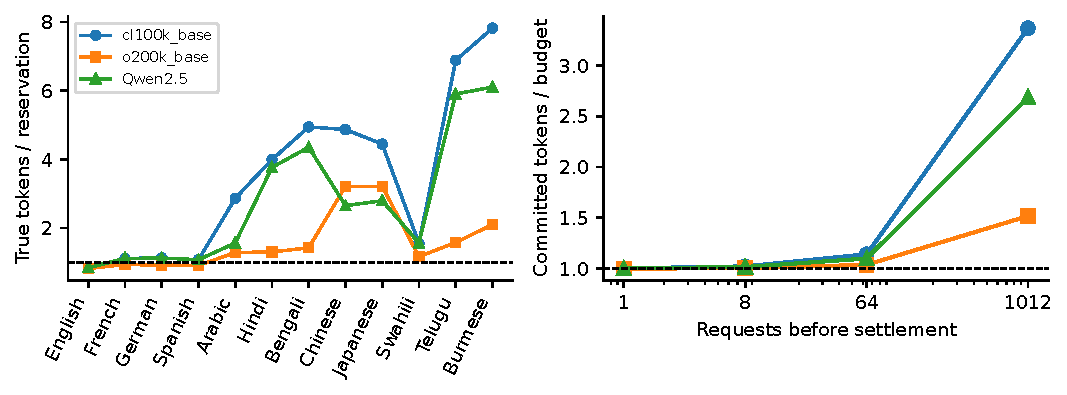
\includegraphics[width=.98\linewidth]{../figures/ledger_error.pdf}
\caption{Left: mean exact input tokens divided by mean character reservation, by language. Right: aggregate committed usage divided by the fixed aggregate budget as settlement is delayed. Dashed lines mark agreement or full budget. The three curves use the same text and admission policy but different exact token units.}
\Description{Tokenizer-dependent character-estimation error is largest for several non-Latin scripts. Quota overcommitment grows as more requests are admitted before settlement.}
\label{fig:error}
\end{figure}

\subsection{RQ2: Exact Accounting Exposes an Entitlement Gap}
Exact reservations restore per-key feasibility in every tested condition. They do not restore comparable-task access. At the central budget, the mean access gaps are 45.80 points for cl100k\_base, 34.32 for o200k\_base, and 44.59 for Qwen2.5. The minimum coverages are approximately 4.32\%, 15.83\%, and 5.63\%. These are differences under a specifically chosen equal-token entitlement policy, not measures of unequal treatment by the model's generated answers.

Bytes offers another capacity-safe policy. Its smaller numerical gaps, around eight percentage points, accompany mean admission near 7\% for every tokenizer and aggregate utilization between 20.5\% and 39.3\%. A conservative language-agnostic upper bound can therefore produce a superficially small access gap by admitting little work. Reporting minimum coverage and utilization prevents interpreting that result as an unqualified fairness improvement. Exact token counting is the appropriate compliance control when the tokenizer and request representation are available; byte reservation is a deliberately conservative diagnostic baseline.

\subsection{RQ3: Calibrating Entitlements Improves Minimum Access at a Cost}
At the same aggregate budget, calibration reduces the central gap to 0.56, 1.03, and 0.76 points for the three tokenizer units. The corresponding minimum coverages rise to 12.93\%, 30.90\%, and 15.89\%. Held-out access is close to, but not exactly, equal because development means are imperfect predictors of held-out cost and the admission process is discrete. Table~\ref{tab:bootstrap} shows that the central contrast remains large under paired sentence resampling.

\begin{table}[t]
\centering\small\begin{tabular}{lrrr}\toprule
Tokenizer & Gap reduction (pp) & Throughput ratio & Minimum access (\%)\\\midrule
cl100k\_base & [43.18, 46.84] & [0.573, 0.624] & [11.96, 13.74]\\
o200k\_base & [31.32, 34.85] & [0.916, 0.937] & [29.25, 32.11]\\
Qwen2.5 & [41.76, 45.65] & [0.579, 0.628] & [14.82, 16.90]\\
\bottomrule\end{tabular}

\caption{Paired sentence-bootstrap sensitivity intervals, central burst condition, 1,000 replicates per tokenizer. Gap reduction compares Exact with Calibrated. Throughput ratio is Calibrated/Exact. Minimum access refers to Calibrated. The percentile adjustment covers three tokenizer comparisons for each statistic, conditional on this benchmark.}
\label{tab:bootstrap}
\end{table}

The cost is material. Calibration admits 59.6\%, 92.7\%, and 60.2\% as many requests as exact equal quotas, respectively, when comparing the ratios of mean admitted requests in Table~\ref{tab:main}. Thus the reduction is approximately 40.4\%, 7.3\%, and 39.8\%. It is inappropriate to claim free fairness gains. Equal aggregate tokens can fund fewer tasks when quota shifts toward expensive translations. The relevant decision is whether that redistribution fulfills a justified service commitment.

The calibrated minimum coverage also tracks the exact common-prefix benchmark (Figure~\ref{fig:frontier}). At the central quota, mean prefix coverages are 13.17\%, 31.39\%, and 16.16\%. Their closeness indicates that separate-data calibration captures much of the cost variation for this corpus; it does not establish equality to an optimal online policy. The cheapest-count bounds are considerably larger: 22.53\%, 44.47\%, and 26.58\%. Achieving those upper counts permits choosing different inexpensive tasks in each language, and therefore changes the service being compared.

\begin{figure}[t]
\centering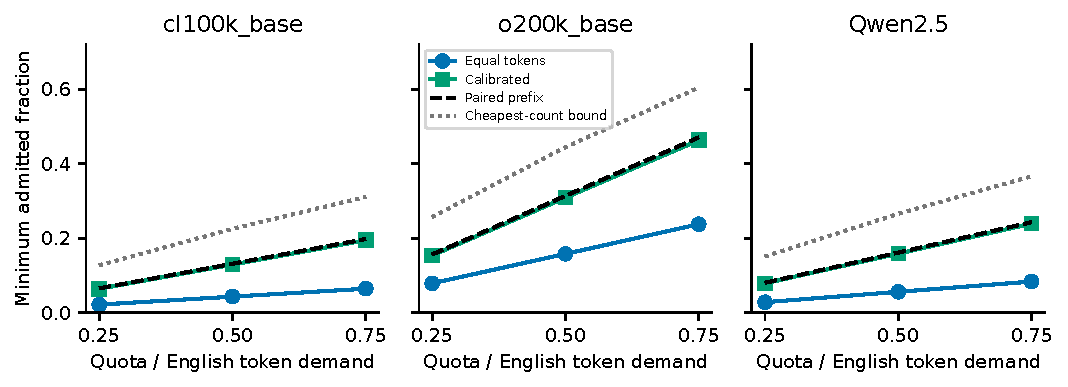
\includegraphics[width=.98\linewidth]{../figures/frontier.pdf}
\caption{Minimum coverage across three quota pressures. Exact equal quotas, calibrated quotas, a common translated-task prefix, and the cheapest-task equal-count frontier use the same aggregate budget. The dotted bound permits content selection; it is not evidence that the same tasks could receive that coverage.}
\Description{Calibration follows the common-prefix benchmark closely. A benchmark that admits the cheapest tasks in each language attains higher count parity but changes task identity. Equal token quotas have lower minimum access.}
\label{fig:frontier}
\end{figure}

\subsection{Robustness, Calibration Error, and Execution Checks}
The four-sentence document check retains the pattern. At the central burst quota, Chars/4 aggregate ratios are 3.316, 1.492, and 2.647, while calibrated gaps are 0.66, 1.20, and 0.79 percentage points. It is a length check on the same source corpus, not cross-domain replication. All main budget levels and both timing endpoints are released in the results, including conditions that have weaker effects.

Calibration is not robust to arbitrary policy or distribution changes. Multiplying every non-English weight by 0.75 raises central gaps to 4.65, 10.83, and 5.70 points. Multiplying those weights by 1.25 yields 2.96, 6.84, and 3.68 points. In the English-priority stress case, minimum access falls to 6.60\%, 16.26\%, and 8.16\% and gaps exceed 83 points. This condition deliberately redistributes half the pool to English despite balanced translated demand. It demonstrates that calibration is an entitlement decision whose priorities can dominate tokenizer improvements; it does not estimate observed traffic imbalance.

All eight test functions pass. All 291,456 Lua admission decisions match the simulator, and final settled counters match exactly across the 24 Redis conditions. This rules out a replay translation error for those conditions. It does not validate omitted HTTP paths, mixed failures, production routing, window rollover, or deployed usage distributions. The strongest empirical conclusion is the existence and measured magnitude of the mechanism in an executable component configuration, together with reproducible capacity-feasible alternatives.

\section{Accountability and Deployment Implications}
\subsection{Audit Both the Unit and the Boundary}
A quota policy can be syntactically language-blind while depending on a language-sensitive measurement function. The gateway operator chooses which estimator determines admission and when true usage changes the counter. The tokenizer provider chooses the token unit. The product owner chooses whether an equal quota is meant to buy equal resource units, equal opportunities to submit comparable content, or some other service promise. These decisions should not be collapsed into a single model fairness score.

We recommend reporting a quota audit record with five linked fields: tokenizer and representation version; reservation estimator and output assumptions; settlement timing and retry behavior; entitlement allocation and parent limits; and access metrics paired with both aggregate and per-key quota utilization. The record must also state the workload denominator. A translated-input denominator is suitable for a controlled linguistic-access comparison, while unrelated real customer workloads would require domain and purpose information before supporting the same inference. These records make it possible to identify whether a proposed improvement changes measurement, capacity, or distribution of entitlements.

Correcting an estimator can look like worsening fairness because some customers receive fewer admissions afterward. That possibility does not justify preserving under-reservation. It means the correction should be evaluated separately from the decision about who receives the now-enforced capacity. Our experiment shows the distinction concretely: exact accounting fixes compliance, while entitlement calibration addresses a different access objective and requires a transfer of capacity. Procurement and internal governance can require both claims to be supported separately.

\subsection{Practical Applications and Institutional Choices}
The immediate application is quality assurance for multilingual document-indexing and retrieval products, API gateways, and enterprise usage plans. Operators can run translated probes before changing a tokenizer, estimation rule, or concurrency setting. Regression tests should flag both admission inversions and hidden overcommitment. An access claim should identify who bears the difference: customers through fewer completed tasks, providers through additional capacity, or other customers through redistributed entitlements. Our calibration experiment preserves the last accounting total but explicitly shifts capacity between keys.

A commercial audit tool could package versioned tokenizer measurement, ledger conformance checks, workload-sensitive quota configuration, and an evidence report. This is a plausible implementation use, not evidence of market demand, patentability, or defensible intellectual-property novelty. A service promising equal-price multilingual processing might instead fund greater total capacity, choose more balanced tokenizers, change pricing, or define workload-specific entitlements. The study measures some technical consequences of these choices; it does not establish which allocation a community should accept.

Language labels should not automatically become personal classifications or punitive controls. People switch languages, use mixed scripts, and share devices and accounts. A deployed weighting system based on inferred language could introduce new privacy risks, manipulation opportunities, or exclusion of unrecognized varieties. Safer applications include voluntary workload classes, transparent task-based plans, and testing of aggregate product commitments. Any per-user assignment mechanism requires independent evaluation, including contestability and an explanation of what the assigned class changes.

\section{Limitations}
Our evidence supports a restricted, reproducible mechanism. First, FLORES translations control much of the input content but come from a limited collection of web articles. They do not represent all dialects, code-switching, disability-related interaction patterns, long legal documents, or observed customer arrivals. Translation quality varies, and equivalence of source task identity is not equivalence of downstream model utility. We have not measured service quality, comprehension, refusal rates, or successful user outcomes.

Second, the study is input-only. Generation caps, actual output lengths, tokenizer-specific chat framing, hidden provider processing, cache accounting, multimodal costs, tool interactions, and retries can change reservations and usage. No conclusion about those paths follows from our counts. Full-burst settlement is an intentional stress endpoint, not an estimate of typical concurrency. Serial and intermediate blocks show the dependence on timing, but omit real latency distributions and overlapping quota windows.

Third, component execution is narrower than deployment evaluation. The pinned gateway file explicitly carries development status. AST extraction and unchanged Lua execution verify the relevant computations, but do not demonstrate that all deployed configurations reach them. We have not tested the whole proxy or a live hosted provider. Source updates may change the result. The artifact pins the revision to make that limitation testable.

Fourth, equal translated-task access is a chosen normative objective. Equal resource entitlements might be the appropriate promise in some settings; language-aware transfers might be inappropriate or insufficient in others. Our worst-language gap treats each selected language equally and is sensitive to the language set. There are no inferred demographic identities or population-weighted welfare claims. The dramatic throughput tradeoff with two tokenizer units is a reason to expose the allocation decision, not to hide it behind a fairness label.

Finally, the calibration baseline has no guarantee under arbitrary distribution shift, unknown tokenization, or strategic workload labeling. Its weights are means from a nearby translated-text split. The separate-data design prevents fitting those means directly to the evaluation set but does not establish generalization to production. Literature searches cannot prove the absence of every earlier treatment of a related mechanism. Our contribution claim is bounded to the combined audit protocol, component evidence, and comparative results described here; its conceptual ingredients have explicit precedents.

\section{Conclusion}
Multilingual quota audits need to distinguish the units reserved before admission, the tokens committed by accepted inputs, and the comparable tasks that receive access. In a pinned gateway component, a character-based estimate changes language admission rankings and can commit substantially more tokens than the quota permits before reconciliation. Exact counting restores accounting compliance while revealing large access differences under equal token entitlements. Separate-data entitlement calibration reduces those differences at a fixed total quota, with substantial and tokenizer-dependent request-throughput costs. A credible access improvement must state which service objective it serves, respect the capacity constraint used in the comparison, and expose who receives the redistributed resource.

\clearpage
\section*{Ethical Considerations and Adverse Impacts}
The released measurements contain sentence identifiers, language codes, aggregate counts, and controlled admission outcomes. Public translations are retrieved from their original licensed distribution; the repository does not republish the corpus text. The study makes no attribution of intent or claim about the prevalence of harm at a vendor or customer deployment. A source-level result should not be used to characterize an entire service without checking its configured execution path.

The intervention redistributes a fixed token pool. It can improve a chosen minimum-access objective while reducing total admitted requests and restricting access for previously advantaged workloads. This tradeoff is reported explicitly. In deployment, assigning language classes can itself be harmful, particularly for mixed-language users and unrecognized varieties. Our known corpus labels are not evidence that language inference is appropriate for personal allocation decisions. Auditing should support transparent product commitments and contestable policies rather than new opaque classifications.

\section*{Generative AI Usage Statement}
Codex (GPT-6) was used substantively to develop the research framing, search and structure related literature, write and execute analysis code and tests, produce figures, interpret experimental outputs, and draft and revise the manuscript. This statement does not represent that independent human verification of every claim has occurred. The human author retains responsibility for the originality, accuracy, integrity, and submission of the work. The artifact records executable methods and results so that the reported claims can be checked independently.

\clearpage
\bibliographystyle{ACM-Reference-Format}
\bibliography{references}
\appendix
\section{Reproducibility Specification}
The reference artifact records the upstream source hash, tokenizer revision and package versions, original-data file hashes, the prospective local protocol, raw token-count tables, all replay summaries, bootstrap replicates, Redis decision digests, and figure-generation code. Data retrieval and tokenization are separate from replay so that admission experiments can be reproduced directly from count tables without loading model weights or contacting a model API. The named manuscript can include an author-linked repository; the anonymous manuscript omits identifying repository links.

To reproduce from counts, create a Python environment with the recorded dependencies and run \texttt{python -m pytest -q tests}, \texttt{python scripts/run.py}, \texttt{python scripts/uncertainty.py}, and \texttt{python scripts/figures.py}. With Redis installed, \texttt{python scripts/redis\_check.py} starts an isolated, nonpersistent server and terminates it after validation. Tokenization can be regenerated with \texttt{scripts/prepare.py} and the original FLORES-200 archive. The four-sentence check uses \texttt{scripts/blocks.py}. The source package includes the upstream MIT license and distinguishes the upstream code from the audit implementation.

\begin{table}[h]
\centering\small
\begin{tabular}{ll}\toprule
Object & Specification\\\midrule
Primary text unit & One FLORES-200 sentence; aligned by split and row index\\
Calibration / evaluation sizes & 997 / 1,012 sentence IDs per language\\
Language set & eng\_Latn, fra\_Latn, deu\_Latn, spa\_Latn, arb\_Arab, hin\_Deva\\
 & ben\_Beng, zho\_Hans, jpn\_Jpan, swh\_Latn, tel\_Telu, mya\_Mymr\\
Output tokens & Zero; input-only accounting\\
Order seeds & 100--129; same permutation across languages and policies\\
Quota pressure & $f=0.25,0.5,0.75$; fixed total budget within each condition\\
Settlement blocks & 1 and 1,012; additionally 8 and 64 at $f=0.5$\\
Bootstrap & 1,000 paired sentence resamples per tokenizer; seed 2026\\
Redis validation & Two complete orders; 24 conditions; 291,456 decisions\\\bottomrule
\end{tabular}
\caption{Compact reproduction specification. The main simulation is a controlled quota experiment, not a production traffic trace.}
\end{table}

\section{Additional Proof and Implementation Details}
For the serial bound, let $S\leq B$ be usage just before the first request that crosses the quota after settlement. Admission gives $S+r\leq B$. Settled usage is $S+c\leq B+(c-r)_+$. Since future reservations are positive and the counter is already above $B$, no later request can be admitted in that unexpired window. If no crossing occurs, the bound is trivial. This argument explains why frequent reconciliation changes the magnitude of an under-reservation failure without making the estimator uniformly safe.

For exact equal-count feasibility, the cheapest $k$ costs in a language minimize the cost of any $k$-element subset by an exchange argument: replacing a chosen expensive item with an unchosen cheaper item cannot increase cost. Because each language's selection is independent under the pooled budget, their minima add. The exhaustive checker independently enumerates all $2^8$ selections in each of forty four-task, two-language instances and checks the greatest feasible minimum count against Equation~\eqref{eq:count}.

The replay maintains one integer vector for counters and one for unsettled signed deltas. Within a batch, admission updates the reservation counter; at the batch boundary the signed deltas replace reservations with true demand. The resulting counter is asserted equal to the sum of exact costs of all admitted requests. Lua validation repeats each key's ordered stream using the upstream check script, then applies the corresponding signed reconciliation deltas with the observed window identity. It compares every admission bit and final counter, not just mean coverage. The Redis tests exercise one descriptor per key and no window rollover; they do not certify cross-descriptor rollback behavior.

\ifdefined\namedversion
\section{Author Artifact}
Code and results: \url{https://github.com/shi1720/quota-ledger-audit}. This link is intentionally excluded from the anonymous manuscript.
\fi
\end{document}
